\chapter*{ECRICOME 2018 : le sujet}
  
%

\section*{Exercice I}

\subsection*{Partie I}

\begin{noliste}{1.}
  \setlength{\itemsep}{4mm}
\item Soit $A$ la matrice de $\M{3}$ donnée par : $A =
  \begin{smatrix}
    2 & 1 & -2\\
    0 & 3 & 0\\
    1 & -1 & 5
  \end{smatrix}
  $.
  \begin{noliste}{a)}
    \setlength{\itemsep}{2mm}
  \item Calculer $A^{2}-7A$.

    

  \item En déduire que les seuls réels susceptibles d'être valeurs
    propres de $A$ sont les réels $3$ et $4$.

    


    %\newpage


  \item Trouver alors toutes les valeurs propres de $A$, et pour
    chacune d'entre elles, donner une base du sous-espace propre
    associé.

    

  \item La matrice $A$ est-elle inversible ? Est-elle diagonalisable ?

    

  \end{noliste}

\item Soit $\B = (e_{1},e_{2},e_{3})$ la base canonique de $\R^{3}$ et
  $f$ l'endomorphisme de $\R^{3}$ dont la matrice représentative dans
  la base $\B$ est la matrice : $B =
  \begin{smatrix}
    1 & -1 & -1\\
    -3 & 3 & -3\\
    -1 & 1 & 1
  \end{smatrix}
  $.
  \begin{noliste}{a)}
    \setlength{\itemsep}{2mm}
  \item Déterminer le noyau de $f$. En déduire une valeur propre de
    $f$ et l'espace propre associé.

    

  \item Déterminer le rang de la matrice $B-2I_{3}$.

    

  \item Calculer $f(e_{1} - e_{2} - e_{3})$.

    
    
  \item Déduire des questions précédentes que l'endomorphisme $f$ est
    diagonalisable.

    
  \end{noliste}
  
\item Trouver une matrice $P$ inversible vérifiant toutes les
  conditions ci-dessous :
  \begin{noliste}{$\star$}
  \item la matrice $D_{2} = P^{-1} \ B \ P$ est égale à
    $\begin{smatrix}
      3 & 0 & 0\\
      0 & 0 & 0\\
      0 & 0 & 2
    \end{smatrix}
    $,
  \item les coefficients situés sur la première ligne de $P$ sont $1$,
    $1$ et $-1$ (de gauche à droite),
  \item la matrice $D_{1} = P^{-1}\ A \ P$ est également diagonale.
  \end{noliste}

  
\end{noliste}

\subsection*{Partie II} 

\noindent
On pose $X_{0} =
\begin{smatrix}
  3\\
  0\\
  -1
\end{smatrix}
$, $X_{1} = 
\begin{smatrix}
  3\\
  0\\
  -2
\end{smatrix}
$, et pour tout entier naturel $n$ : $X_{n + 2} = \dfrac{1}{6} \ A \
X_{n + 1} + \dfrac{1}{6} \ B \ X_{n}$. \\
Soit $(Y_{n})_{n \in \N}$ la suite matricielle définie par : $\forall
n \in \N, \ Y_{n} = P^{-1} X_{n}$.
\begin{noliste}{1.}
  \setlength{\itemsep}{4mm}
\item Démontrer que : $\forall n \in \N $, $Y_{n + 2} = \dfrac{1}{6} \
  D_{1} \ Y_{n + 1} + \dfrac{1}{6} \ D_{2} \ Y_{n}$.

  

\item Pour tout entier naturel $n$, on note $Y_{n} =
  \begin{smatrix}
    a_{n}\\
    b_{n}\\
    c_{n}
  \end{smatrix}
  $.\\
  Déduire de la question précédente que :
  \[
  \forall n \in \N, \ \left\{
    \begin{array}{ll}
      a_{n + 2} & = \dfrac{1}{2} \ a_{n + 1} + \dfrac{1}{2} \ a_{n}\\
      & \\
      b_{n + 2} & = \dfrac{1}{2} \ b_{n + 1}\\
      & \\
      c_{n + 2} & = \dfrac{2}{3} \ c_{n + 1} + \dfrac{1}{3} \ c_{n}
    \end{array}
  \right.
  \]

\newpage  

\item Démontrer que $P^{-1} =
  \begin{smatrix}
    1 & -1 & 1\\
    1 & 0 & 1\\
    1 & -1 & 2
  \end{smatrix}
  $, puis calculer les matrices $Y_{0}$ et $Y_{1}$.

  

\item Pour tout entier naturel $n$, calculer $a_{n}$, $b_{n}$ et
  $c_{n}$ en fonction de $n$.

  
  
\item En déduire l'expression de $X_{n}$ en fonction de $n$, pour tout
  entier naturel $n$.\\
  On notera $X_{n} =
  \begin{smatrix}
    \alpha_{n}\\
    \beta_{n}\\
    \gamma_{n}
  \end{smatrix}
  $, et on vérifiera que :
  \[
  \beta_{n} = \left( \dfrac{1}{2} \right)^{n-1} - \dfrac{2}{3} \left(-
    \dfrac{1}{2} \right)^{n} - \dfrac{4}{3}
  \]

  

\item
  \begin{noliste}{a)}
    \setlength{\itemsep}{2mm}
  \item Compléter la fonction ci-dessous qui prend en argument un
    entier $n$ supérieur ou égal à $2$ et qui renvoie la matrice
    $X_{n}$ :\\[-.2cm]
    \begin{scilab}
      & \tcFun{function} \tcVar{res} = \underline{X}(\tcVar{n}) \nl %
      & \qquad Xold = [3; 0; -1]  \nl %
      & \qquad Xnew = [3; 0; -2] \nl %
      & \qquad A = [2,1,-2; 0,3,0; 1,-1,5] \nl %
      & \qquad B = [1,-1,-1; -3,3,-3; -1,1,1] \nl %
      & \qquad \tcFor{for} i = 2:\tcVar{n} \nl %
      & \qquad \qquad Aux = .......... \nl %
      & \qquad \qquad Xold = ......... \nl %
      & \qquad \qquad Xnew = ......... \nl %
      & \qquad \tcFor{end} \nl %
      & \qquad res = ......... \nl %
      & \tcFun{endfunction}       
    \end{scilab}

    

  \item La fonction précédente a été utilisée dans un script
    permettant d'obtenir graphiquement (voir figure 1) les valeurs de
    $\alpha_{n}$, $\beta_{n}$ et $\gamma_{n}$ en fonction de $n$.\\
    Associer chacune des trois représentations graphiques à chacune
    des suites $(\alpha_{n})_{n\in \N}$, $(\beta_{n})_{n\in \N}$,
    $(\gamma_{n})_{n\in \N}$ en justifiant votre réponse.
    \begin{figure}[!h]
      \centering
      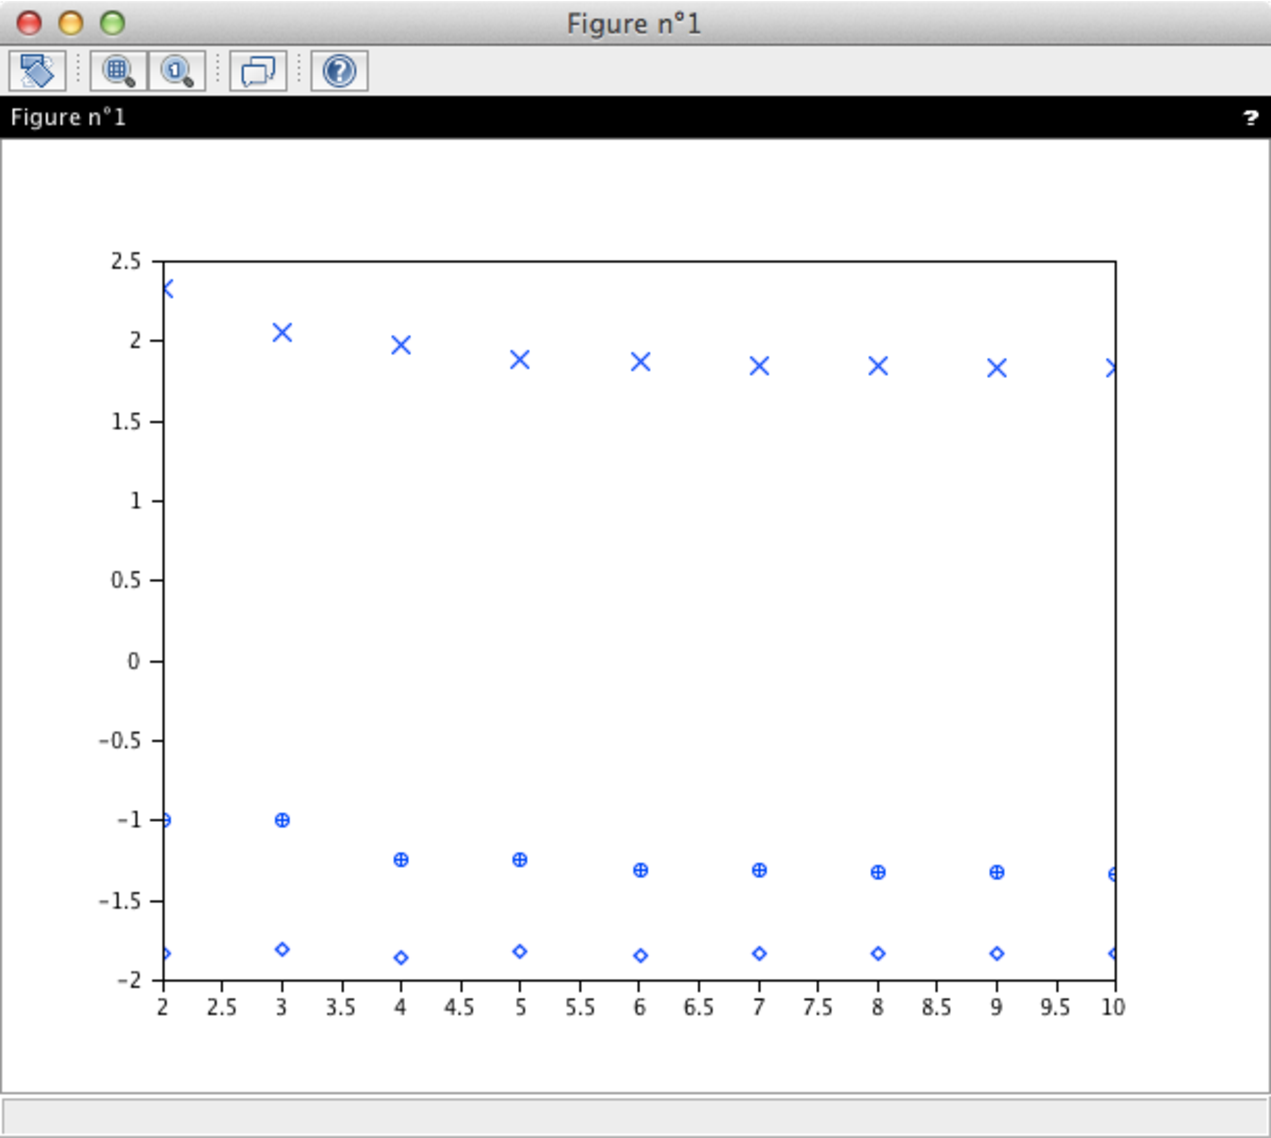
\includegraphics[width=10cm,
      height=8cm]{Figures/ECRICOME_2018/suites_alpha_beta_gamma.pdf}  
    \end{figure}
    % \caption{}
    % \label{fig:nuage}
    
  \end{noliste}
\end{noliste}


\newpage


\section*{Exercice 2}

\subsection*{Partie I : Étude de deux suites}

\noindent
Pour tout entier naturel $n$ non nul, on pose : \ $u_{n} = \Sum{k =
  1}{n} \dfrac{1}{k} - \ln(n)$ \ et \ $v_{n} = u_{n} - \dfrac{1}{n}$.

\begin{noliste}{1.}
 \setlength{\itemsep}{4mm}
\item Soit $f$ la fonction définie sur $\R_+^*$ par $f(x) =
  \dfrac{1}{x + 1} + \ln(x)-\ln(x + 1)$.
  \begin{noliste}{a)}
    \setlength{\itemsep}{2mm}
  \item Déterminer $ \dlim{x \to 0} f(x)$ et $ \dlim{x \to + \infty}
    f(x)$.

    

  \item Étudier les variations de la fonction $f$ sur $\R_+^*$ et
    dresser son tableau de variations.

    

  \item Démontrer que : \ $\forall n \in \N^*, \ u_{n + 1}-u_{n} =
    f(n)$.

    


    %\newpage


  \item En déduire la monotonie de la suite $(u_{n})_{n\in \N^*}$.

    

  \item Écrire une fonction d'en-tête : {\tt function y = u(n)} qui
    prend en argument un entier naturel $n$ non nul et qui renvoie la
    valeur de $u_{n}$.

    
  \end{noliste}


  %\newpage


\item 
  \begin{noliste}{a)}
    \setlength{\itemsep}{2mm}
  \item Montrer que : $\forall n \in \N^*$, $v_{n + 1}-v_{n} =
    \dfrac{1}{n} - \ln \left(1 + \dfrac{1}{n} \right)$.

    

  \item Montrer que pour tout réel $x$ positif : $\ln(1 + x) \leq x$.\\
    En déduire que la suite $(v_{n})_{n \in \N^*}$ est croissante.

    

  \item Donner le développement limité d'ordre 2 de $\ln(1 + x)$ en
    $0$. En déduire que :
    \[
    v_{n + 1}-v_{n} \underset{n\to + \infty}{\sim} \frac{1}{2n^{2}}
    \]
  \end{noliste}

  
  

  %\newpage


  \begin{noliste}{a)}    
    \setcounter{enumii}{3}
  \item Déterminer la nature de la série de terme général $v_{n +
      1}-v_{n}$. On note $\gamma = \Sum{n = 1}{+ \infty}(v_{n +
      1}-v_{n})$.

    

  \item Pour $n \geq 2$, simplifier la somme partielle : \ $ \Sum{k =
      1}{n-1} (v_{k + 1}-v_{k})$.\\
    En déduire que la suite $(v_{n})_{n \geq 2}$ converge vers
    $\gamma$.

    

  \end{noliste}

\item 
  \begin{noliste}{a)} 
    \setlength{\itemsep}{2mm}
  \item Déterminer $ \dlim{n \to \infty} u_{n}$.

    

  \item Montrer que :
    \[
    \forall n \in \N^*, \ v_{n} \leq \gamma \leq u_{n}
    \]
    puis que :
    \[
    \forall n \in \N^*, \ \big|u_{n} - \gamma\big| \leq \dfrac{1}{n}
    \]

    

  \item On rappelle que l'instruction {\tt floor(x)} renvoie la partie
    entière d'un réel $x$ et on suppose que la fonction {\tt u} de la
    question \itbf{1.e)} a été correctement programmée. Expliquer
    l'intérêt et le fonctionnement du script ci-dessous :
    \begin{scilab}
      & eps = input(\ttq{}Entrer un réel strictement positif : \ttq{})
      \nl %
      & n = floor(1/eps) + 1 \nl %
      & disp(u(n))
    \end{scilab}

    
  \end{noliste}
\end{noliste}


\newpage


\section*{Partie II : Étude d'une série}

\noindent
Pour tout entier naturel $n$, on pose \ $a_{n} = \dfrac1{n(2n-1)}$.
\begin{noliste}{1.}
  \setlength{\itemsep}{4mm}
\item Démontrer que la série de terme général $a_{n}$ converge.

  

\item
  \begin{noliste}{a)} 
    \setlength{\itemsep}{2mm}
  \item Justifier que : $\forall n \in \N^*, \ \Sum{k = 1}{n}
    \dfrac{1}{2k-1} = \Sum{k = 1}{2n} \dfrac{1}{k} - \Sum{k = 1}{n}
    \dfrac{1}{2k}$.
    
    

  \item Déterminer deux réels $\alpha$ et $\beta$ tels que : $\forall
    n \in \N^*, \ a_{n} = \dfrac{\alpha}{n} + \dfrac{\beta}{2n-1}$.

    

  \item En déduire que : $\forall n \in \N^*$, $\Sum{k = 1}{n} a_{k} =
    2 \Sum{k = n + 1}{2n} \dfrac{1}{k}$.

    
  \end{noliste}


  %\newpage


\item 
  \begin{noliste}{a)}
    \setlength{\itemsep}{2mm}
  \item Montrer que : 
    \[
    \forall n \in \N^*, \ \Sum{k = n + 1}{2n} \dfrac{1}{k} =
    u_{2n}-u_{n} + \ln(2)
    \]
    où $(u_{n})_{n \in \N^*}$ est la suite définie dans la partie I.

    

  \item Calculer alors  $\Sum{k = 1}{+ \infty} a_{k}$.
    
    
  \end{noliste}

\item 
  \begin{noliste}{a)}
    \setlength{\itemsep}{2mm}
  \item Montrer que : $\forall n \in \N^*, \ \Sum{k = n + 1}{2n}
    \dfrac{1}{k} = \dfrac{1}{n} \ \Sum{k = 1}{n} \dfrac{1}{1 +
      \frac{k}{n}}$.

    


    %\newpage


  \item Retrouver alors le résultat de la question \itbf{3.b)}.

    

  \end{noliste}
\end{noliste}

\section*{Exercice 3}

\noindent
Soit $n$ un entier naturel non nul.\\
Dans une fête foraine, un stand propose le jeu suivant : le joueur
lance $n$ fois une pièce et compte le nombre de Pile obtenus. Si ce
nombre est pair, le joueur est déclaré vainqueur, et s'il est impair,
il est déclaré perdant.\\
Si le joueur est déclaré vainqueur, il gagne 10 euros pour chaque Pile
obtenu, mais s'il a perdu, il doit payer 10 euros pour chaque Pile
obtenu.\\
En particulier, s'il n'obtient aucun Pile, il est déclaré vainqueur,
mais ne remporte rien. La pièce est truquée, et à chaque lancer, la
probabilité d'obtenir Pile est égale à $p$ ($p \in \ ]0,1[$), et celle
d'obtenir Face est de $1-p$.\\
On notera $X$ la variable aléatoire égale au nombre de Pile obtenus,
et $G$ la variable aléatoire égale au gain algébrique du joueur.\\
Enfin, on notera $A$ l'événement : \og le joueur est déclaré
vainqueur \fg{} et on dira que le jeu est favorable au joueur si
l'espérance mathématique de la variable aléatoire $G$ est positive.



%\newpage


\subsection*{Partie I}
 
\noindent
Dans cette partie, on suppose que $n = 3$ et $p = \dfrac{2}{3}$.
\begin{noliste}{1.}
  \setlength{\itemsep}{4mm}
\item Reconnaître la loi de $X$ et vérifier que : $\Prob\left(A\right)
  = \dfrac{13}{27}$.

  

\item Montrer que : $G(\Omega) = \{-30, -10, 0, 20\}$, puis expliciter
  la loi de $G$.

  

\item Calculer l'espérance de $G$. Le jeu est-il favorable au joueur ?
  
  
\end{noliste}


\newpage


\subsection*{Partie II}

\noindent
Dans cette partie, on revient au cas général, où $n$ est entier
naturel non nul et $p \in \ ]0,1[$.\\
Celui qui tient le stand souhaite rendre le jeu plus attractif en
affichant \og À ce jeu, il y a plus de gagnants que de perdants ! \fg,
et cherche donc les conditions nécessaires sur $p$ et $n$ pour que son
affichage ne soit pas mensonger.\\
Soit $Y$ la variable aléatoire définie par : $Y = (-1)^{X}$.\\
Autrement dit, $Y$ prend la valeur $1$ lorsque $X$ prend une valeur
paire, et $Y$ prend la valeur $-1$ lorsque $X$ prend une valeur
impaire.
\begin{noliste}{1.}
  \setlength{\itemsep}{4mm}
\item
  \begin{noliste}{a)} 
    \setlength{\itemsep}{2mm}
  \item On note $Z = \dfrac{Y + 1}{2}$.\\[.2cm]
    Déterminer $Y(\Omega)$, puis montrer que $Z$ suit une loi de
    Bernoulli de paramètre $\Prob\left( A \right)$.

    

  \item Démontrer que : $\E(Y) = 2 \Prob(A) - 1$.

    
  \end{noliste}


  %\newpage


\item 
  \begin{noliste}{a)}
    \setlength{\itemsep}{2mm}
  \item Donner la loi de $X$.

    

  \item En déduire que l'on a également : 
    \[
    \E(Y) = \Sum{k = 0}{n} (-1)^{k} \dbinom{n}{k} p^{k}(1-p)^{n-k}
    \]
    puis que : $\E(Y) = (1-2p)^{n}$.

    
  \end{noliste}

\item Exprimer alors la valeur de $\Prob(A)$ en fonction de $n$ et
  $p$.

  


  %\newpage


\item Démontrer que :
  \[
  \Prob\left(A\right) \geq \dfrac{1}{2} \ \Leftrightarrow \ \left[ p
    \leq \dfrac{1}{2} \hbox{ OU \og $n$ est pair \fg{}} \right]
  \]

  

\end{noliste}


%\newpage


\subsection*{Partie III}

\noindent
Le concepteur du jeu souhaite cependant vérifier que, tout en laissant
son jeu attractif (c'est à dire en faisant en sorte que
$\Prob\left(A\right) \geq \dfrac12$ ), son activité soit rentable pour
lui, autrement dit que le jeu soit défavorable au joueur (c'est à dire
que $\E(G) \leq 0$).

\begin{noliste}{1.}
  \setlength{\itemsep}{4mm}
\item Exprimer $G$ en fonction de $X$ et $Y$. En déduire que : $\E(G)
  = 10 \Sum{k = 0}{n} (-1)^{k} \ k \ \Prob\left(\Ev{X = k}\right)$.

  


%  %\newpage


\item Démontrer que : $\forall k \in \llb 1, n\rrb, \ k \
  \dbinom{n}{k} = n \dbinom{n-1}{k-1}$.

  

\item Montrer que : $\E(G) = -10 \ np \ (1-2p)^{n-1}$.

  


  %\newpage


\item Démontrer alors que :
  \[
  \left\{ 
    \begin{array}{r}
      \Prob(A) \geq \dfrac{1}{2} 
      \\[.4cm]
      \E(G) \leq 0
    \end{array}
  \right. \ \Leftrightarrow \ p \leq \dfrac{1}{2}
  \]

  

\item 
  \begin{noliste}{a)} 
    \setlength{\itemsep}{2mm}
  \item Étudier la fonction $f$ définie sur $\left[0, \frac{1}{2}
    \right]$ par : $\forall x \in \left[0, \frac{1}{2} \right], \ f(x)
    = x \ (1-2x)^{n-1}$.

    

  \item Pour une valeur de $n$ fixée, comment le concepteur du jeu
    doit-il truquer sa pièce (c'est à dire quelle valeur doit-il
    donner à $p \in \left[0, \frac{1}{2} \right]$ ) pour optimiser la
    rentabilité de son activité ?

    
  \end{noliste}
\end{noliste}


\newpage


\subsection*{Partie IV}

\noindent
Le forain décide de fixer $n = 2$ et $p = \dfrac{1}{4}$. En période
estivale, il pense pouvoir compter sur la participation de $200$
clients dans le journée. Avant de se décider à installer son stand, il
voudrait être certain, avec un risque d'erreur inférieur à $10 \%$,
qu'il gagnera plus de $100$ euros dans la journée.\\
Pour tout entier $i$ compris ente $1$ et $200$, on note alors $G_{i}$
le gain algébrique du $\eme{i}$ joueur.\\
On note aussi $J$ la variable aléatoire égale au gain du forain sur
toute la journée.
\begin{noliste}{1.}
  \setlength{\itemsep}{4mm}
\item Pour tout entier $i \in \llb 1,200 \rrb$, donner la loi de
  $G_{i}$ et calculer son espérance et sa variance.
  
  

\item Exprimer la variable aléatoire $J$ en fonction des variables
  aléatoires $G_{i}$.\\
  Démontrer alors que $\E(J) = 500$ et $\V(J) = 11250$.

  

\item Justifier que : $\Prob\big(\Ev{ J \leq 100}\big) \leq \Prob\big(
  \Ev{|J-500|\geq 400} \big)$.

  

\item Rappeler l'inégalité de Bienaymé-Tchebychev, puis montrer que :
  $\Prob\left(\Ev{J \leq 100}\right) \leq \dfrac{9}{128}$.

  

\item Compte tenu de ses exigences de rentabilité, le forain peut-il
  installer son stand ?

  
\end{noliste}
